%%%%%%%%%%%%%%%%%%%%%%%%%%%%%%%%%%%%%%%%%12pt: grandezza caratter
                                        %a4paper: formato a4
                                        %openright: apre i capitoli a destra
                                        %twoside: serve per fare un
                                        %   documento fronteretro
                                        %report: stile tesi (oppure book)
\documentclass[12pt,a4paper,openright,twoside]{report}
%
%%%%%%%%%%%%%%%%%%%%%%%%%%%%%%%%%%%%%%%%%libreria per scrivere in italiano
\usepackage[italian]{babel}
%
%%%%%%%%%%%%%%%%%%%%%%%%%%%%%%%%%%%%%%%%%libreria per accettare i caratteri
                                        %   digitati da tastiera come � �
                                        %   si pu� usare anche
                                        %   \usepackage[T1]{fontenc}
                                        %   per� con questa libreria
                                        %   il tempo di compilazione
                                        %   aumenta
% \usepackage[latin1]{inputenc}
\usepackage[utf8]{inputenc} %in alternativa si pu� usare utf8

%
%%%%%%%%%%%%%%%%%%%%%%%%%%%%%%%%%%%%%%%%%libreria per impostare il documento
\usepackage{fancyhdr}
%
%%%%%%%%%%%%%%%%%%%%%%%%%%%%%%%%%%%%%%%%%libreria per avere l'indentazione
%%%%%%%%%%%%%%%%%%%%%%%%%%%%%%%%%%%%%%%%%   all'inizio dei capitoli, ...
\usepackage{indentfirst}
%
%%%%%%%%%libreria per mostrare le etichette
%\usepackage{showkeys}
%
%%%%%%%%%%%%%%%%%%%%%%%%%%%%%%%%%%%%%%%%%libreria per inserire grafici
\usepackage{graphicx}
%
%%%%%%%%%%%%%%%%%%%%%%%%%%%%%%%%%%%%%%%%%libreria per utilizzare font
                                        %   particolari ad esempio
                                        %   \textsc{}
\usepackage{newlfont}
%
%%%%%%%%%%%%%%%%%%%%%%%%%%%%%%%%%%%%%%%%%librerie matematiche
\usepackage{amssymb}
\usepackage{amsmath}
\usepackage{latexsym}
\usepackage{amsthm}
%
\oddsidemargin=30pt \evensidemargin=20pt%impostano i margini
\hyphenation{sil-la-ba-zio-ne pa-ren-te-si}%serve per la sillabazione: tra parentesi
					   %vanno inserite come nell'esempio le parole
%					   %che latex non riesce a tagliare nel modo giusto andando a capo

%
%%%%%%%%%%%%%%%%%%%%%%%%%%%%%%%%%%%%%%%%%comandi per l'impostazione
                                        %   della pagina, vedi il manuale
                                        %   della libreria fancyhdr
                                        %   per ulteriori delucidazioni
\pagestyle{fancy}\addtolength{\headwidth}{20pt}
\renewcommand{\chaptermark}[1]{\markboth{\thechapter.\ #1}{}}
\renewcommand{\sectionmark}[1]{\markright{\thesection \ #1}{}}
\rhead[\fancyplain{}{\bfseries\leftmark}]{\fancyplain{}{\bfseries\thepage}}
\cfoot{}
%%%%%%%%%%%%%%%%%%%%%%%%%%%%%%%%%%%%%%%%%
\linespread{1.3}                        %comando per impostare l'interlinea
%%%%%%%%%%%%%%%%%%%%%%%%%%%%%%%%%%%%%%%%%definisce nuovi comandi

% % Bibliografia alternativa
% \usepackage{natbib}
% \bibliographystyle{alpha}
% \setcitestyle{super,open={[},close={]}}

\usepackage[titletoc,title,toc,page]{appendix} %appendici
\usepackage{pdfpages} %embed di pdf
\usepackage{lscape} %modalit� landscape
\usepackage{float}%posizionamento elementi
\usepackage{hyperref}%url


\begin{document}
\begin{titlepage}
\begin{center}
{{\Large{\textsc{Alma Mater Studiorum $\cdot$ Universit\`a di
Bologna}}}} \rule[0.1cm]{15.8cm}{0.1mm}
\rule[0.5cm]{15.8cm}{0.6mm}
{\small{\bf SCUOLA DI SCIENZE\\
Corso di Laurea in Nome corso di Laurea }}
\end{center}
\vspace{15mm}
\begin{center}
{\LARGE{\bf TITOLO}}\\
\vspace{3mm}
{\LARGE{\bf DELLA}}\\
\vspace{3mm}
{\LARGE{\bf TESI}}\\
\end{center}
\vspace{40mm}
\par
\noindent
\begin{minipage}[t]{0.47\textwidth}
{\large{\bf Relatore:\\
Chiar.mo Prof.\\
NOME RELATORE}}
\end{minipage}
\hfill
\begin{minipage}[t]{0.47\textwidth}\raggedleft
{\large{\bf Presentata da:\\
NOME LAUREANDO}}
\end{minipage}
\vspace{20mm}
\begin{center}
{\large{\bf Sessione\\%inserire il numero della sessione in cui ci si laurea
Anno Accademico }}%inserire l'anno accademico a cui si � iscritti
\end{center}
\end{titlepage}

\begin{titlepage}                       %crea un ambiente libero da vincoli
                                        %   di margini e grandezza caratteri:
                                        %   si pu� modificare quello che si
                                        %   vuole, tanto fuori da questo
                                        %   ambiente tutto viene ristabilit
%
\thispagestyle{empty}                   %elimina il numero della pagina
\topmargin=6.5cm                        %imposta il margina superiore a 6.5cm
\raggedleft                             %incolonna la scrittura a destra
\large                                  %aumenta la grandezza del carattere
                                        %   a 14pt
\em                                     %emfatizza (corsivo) il carattere
Questa � la \textsc{Dedica}:\\
ognuno pu� scrivere quello che vuole, \\
anche nulla \ldots                      %\ldots lascia tre puntini
\newpage                                %va in una pagina nuov
%
%%%%%%%%%%%%%%%%%%%%%%%%%%%%%%%%%%%%%%%%
\clearpage{\pagestyle{empty}\cleardoublepage}%non numera l'ultima pagina sinistra
\end{titlepage}
\pagenumbering{roman}                   %serve per mettere i numeri romani
\chapter*{Introduzione}                 %crea l'introduzione (un capitolo
                                        %   non numerato)
%%%%%%%%%%%%%%%%%%%%%%%%%%%%%%%%%%%%%%%%%imposta l'intestazione di pagina
\rhead[\fancyplain{}{\bfseries
INTRODUZIONE}]{\fancyplain{}{\bfseries\thepage}}
\lhead[\fancyplain{}{\bfseries\thepage}]{\fancyplain{}{\bfseries
INTRODUZIONE}}
%%%%%%%%%%%%%%%%%%%%%%%%%%%%%%%%%%%%%%%%%aggiunge la voce Introduzione
                                        %   nell'indice
\addcontentsline{toc}{chapter}{Introduzione}
Questa � l'introduzione.
%%%%%%%%%%%%%%%%%%%%%%%%%%%%%%%%%%%%%%%%%non numera l'ultima pagina sinistra
\clearpage{\pagestyle{empty}\cleardoublepage}
\tableofcontents                        %crea l'indice
%%%%%%%%%%%%%%%%%%%%%%%%%%%%%%%%%%%%%%%%%imposta l'intestazione di pagina
\rhead[\fancyplain{}{\bfseries\leftmark}]{\fancyplain{}{\bfseries\thepage}}
\lhead[\fancyplain{}{\bfseries\thepage}]{\fancyplain{}{\bfseries
INDICE}}
%%%%%%%%%%%%%%%%%%%%%%%%%%%%%%%%%%%%%%%%%non numera l'ultima pagina sinistra
\clearpage{\pagestyle{empty}\cleardoublepage}
\listoffigures                          %crea l'elenco delle figure
%%%%%%%%%%%%%%%%%%%%%%%%%%%%%%%%%%%%%%%%%non numera l'ultima pagina sinistra
\clearpage{\pagestyle{empty}\cleardoublepage}
\listoftables                           %crea l'elenco delle tabelle
%%%%%%%%%%%%%%%%%%%%%%%%%%%%%%%%%%%%%%%%%non numera l'ultima pagina sinistra
\clearpage{\pagestyle{empty}\cleardoublepage}
\chapter{Primo Capitolo}                %crea il capitolo
%%%%%%%%%%%%%%%%%%%%%%%%%%%%%%%%%%%%%%%%%imposta l'intestazione di pagina
\lhead[\fancyplain{}{\bfseries\thepage}]{\fancyplain{}{\bfseries\rightmark}}
\pagenumbering{arabic}                  %mette i numeri arabi
Questo � il primo capitolo.
\section{Prima Sezione}                 %crea la sezione
Questa � la prima sezione.

Ora vediamo un elenco numerato:         %crea un elenco numerato
\begin{enumerate}
\item primo oggetto
\item secondo oggetto
\item terzo oggetto
\item quarto oggetto
\end{enumerate}

\begin{figure}[h]                       %crea l'ambiente figura; [h] sta
                                        %   per here, cio� la figura va qui
\begin{center}                          %centra nel mezzo della pagina
                                        %   la figura
%\includegraphics[width=5cm]{figura.eps}%inserisce una figura larga 5cm
                                        %se si vuole usare va scommentat
%
%%%%%%%%%%%%%%%%%%%%%%%%%%%%%%%%%%%%%%%%%inserisce la legenda ed etichetta
                                        %   la figura con \label{fig:prima}
\caption[legenda elenco figure]{legenda sotto la figura}\label{fig:prima}
\end{center}
\end{figure}

\section{Seconda Sezione}
Ora vediamo un elenco puntato:
\begin{itemize}                         %crea un elenco puntato
\item primo oggetto
\item secondo oggetto
\end{itemize}

\section{Altra Sezione}
Vediamo un elenco descrittivo:
\begin{description}                     %crea un elenco descrittivo
  \item[OGGETTO1] prima descrizione;
  \item[OGGETTO2] seconda descrizione;
  \item[OGGETTO3] terza descrizione.
\end{description}
%%%%%%%%%%%%%%%%%%%%%%%%%%%%%%%%%%%%%%%%%crea una sottosezione
\subsection{Altra SottoSezione}
%%%%%%%%%%%%%%%%%%%%%%%%%%%%%%%%%%%%%%%%%crea una sottosottosezione
\subsubsection{SottoSottoSezione}Questa sottosottosezione non viene
numerata, ma � solo scritta in grassetto.
\section{Altra Sezione}                 %crea una sottosezione
Vediamo la creazione di una tabella; la tabella \ref{tab:uno}
(richiamo il nome della tabella utilizzando la label che ho messo sotto):
la facciamo di tre righe e tre colonne, la prima colonna
``incolonnata'' a destra (r) e le altre centrate (c):\\
\begin{table}[h]                        %ambiente tabella
                                        %(serve per avere la legenda)
\begin{center}                          %centra nella pagina la tabella
\begin{tabular}{r|c|c}                  %tre colonne con righe verticali
                                        %   prodotte con |
\hline \hline                           %inserisce due righe orizzontali
$(1,1)$ & $(1,2)$ & $(1,3)$\\           %& separa le colonne e con
\hline                                  %inserisce una riga orizzontale
$(2,1)$ & $(2,2)$ & $(2,3)$\\           %  \\ va a capo
\hline                                  %inserisce una riga orizzontale
$(3,1)$ & $(3,2)$ & $(3,3)$\\
\hline \hline                           %inserisce due righe orizzontali
\end{tabular}
\caption[legenda elenco tabelle]{legenda tabella}\label{tab:uno}
\end{center}
\end{table}
\section{Altra Sezione}\label{sec:prova}%posso mettere le label anche
                                        %   alle section
\subsection{Listati dei programmi}
\subsubsection{Primo Listato}
\begin{verbatim}
        In questo ambiente     posso scrivere      come voglio,
lasciare gli spazi che voglio e non % commentare quando voglio
e ci sar� scritto tutto.
Quando lo uso � meglio che disattivi il Wrap del WinEdt
\end{verbatim}

\section{Math mode}
Per inserire simboli matematici (e lettere greche) serve la math mode:

Usando il simbolo del dollaro hai la math mode inline: $5 \times \alpha = 3\lambda$

Altrimenti hai quella con le barre e le quadre \[ \frac{\sum_6^i 3i\theta}{12k^2\times 7}\]

Infine hai quelle con begin equation (che vengono numerate):
\begin{equation}
    \frac{1}{2}\times A_{bcd}\times E^{fgh}
\end{equation}

Anche le equazioni possono avere label.
\section{url e footnote}
per mettere un link usa url: \url{wikipedia.it}

per fare note a pi� di pagina usa footnote\footnote{Tipo questa}


\section{Modalit� landscape}
Se usi landscape la pagina viene girata (nel caso dovessi inserirne una molto grande)
\begin{landscape}
\begin{table}[H]
    \centering
    \begin{tabular}{|c|c|}
    \hline
        \textbf{Numero} & \textbf{\#}  \\ \hline
        UNO & 1  \\ \hline
        DUE & 2  \\ \hline
        TRE & 3  \\ \hline
    \end{tabular}
    \caption{Tabella girata}
    \label{tab:girata}
\end{table}

\end{landscape}
%%%%%%%%%%%%%%%%%%%%%%%%%%%%%%%%%%%%%%%%%non numera l'ultima pagina sinistra
\clearpage{\pagestyle{empty}\cleardoublepage}
%%%%%%%%%%%%%%%%%%%%%%%%%%%%%%%%%%%%%%%%%per fare le conclusioni
\chapter*{Conclusioni}
%%%%%%%%%%%%%%%%%%%%%%%%%%%%%%%%%%%%%%%%%imposta l'intestazione di pagina
\rhead[\fancyplain{}{\bfseries
CONCLUSIONI}]{\fancyplain{}{\bfseries\thepage}}
\lhead[\fancyplain{}{\bfseries\thepage}]{\fancyplain{}{\bfseries
CONCLUSIONI}}
%%%%%%%%%%%%%%%%%%%%%%%%%%%%%%%%%%%%%%%%%aggiunge la voce Conclusioni
                                        %   nell'indice
\addcontentsline{toc}{chapter}{Conclusioni} Queste sono le
conclusioni.\\
In queste conclusioni voglio fare un riferimento alla
bibliografia: questo � il mio riferimento \cite{K3,K4}.


%Appendici alternative ed embed di pdf
% \renewcommand{\appendixtocname}{Appendici}
% \renewcommand{\appendixpagename}{Appendici}
% % \csname @openrightfalse\endcsname
% \pagenumbering{gobble}
% \begin{appendices}
% \chapter{Appendice 1}
% \label{Appendice:A}
% Appendice A

% \chapter{Embed di interi PDF}
% \label{Appendice:B}
% Se ti serve puoi fare embed di PDF interi con pdfpage, scegliendo anche le pagine (o mettendo - se le vuoi tutte):

% 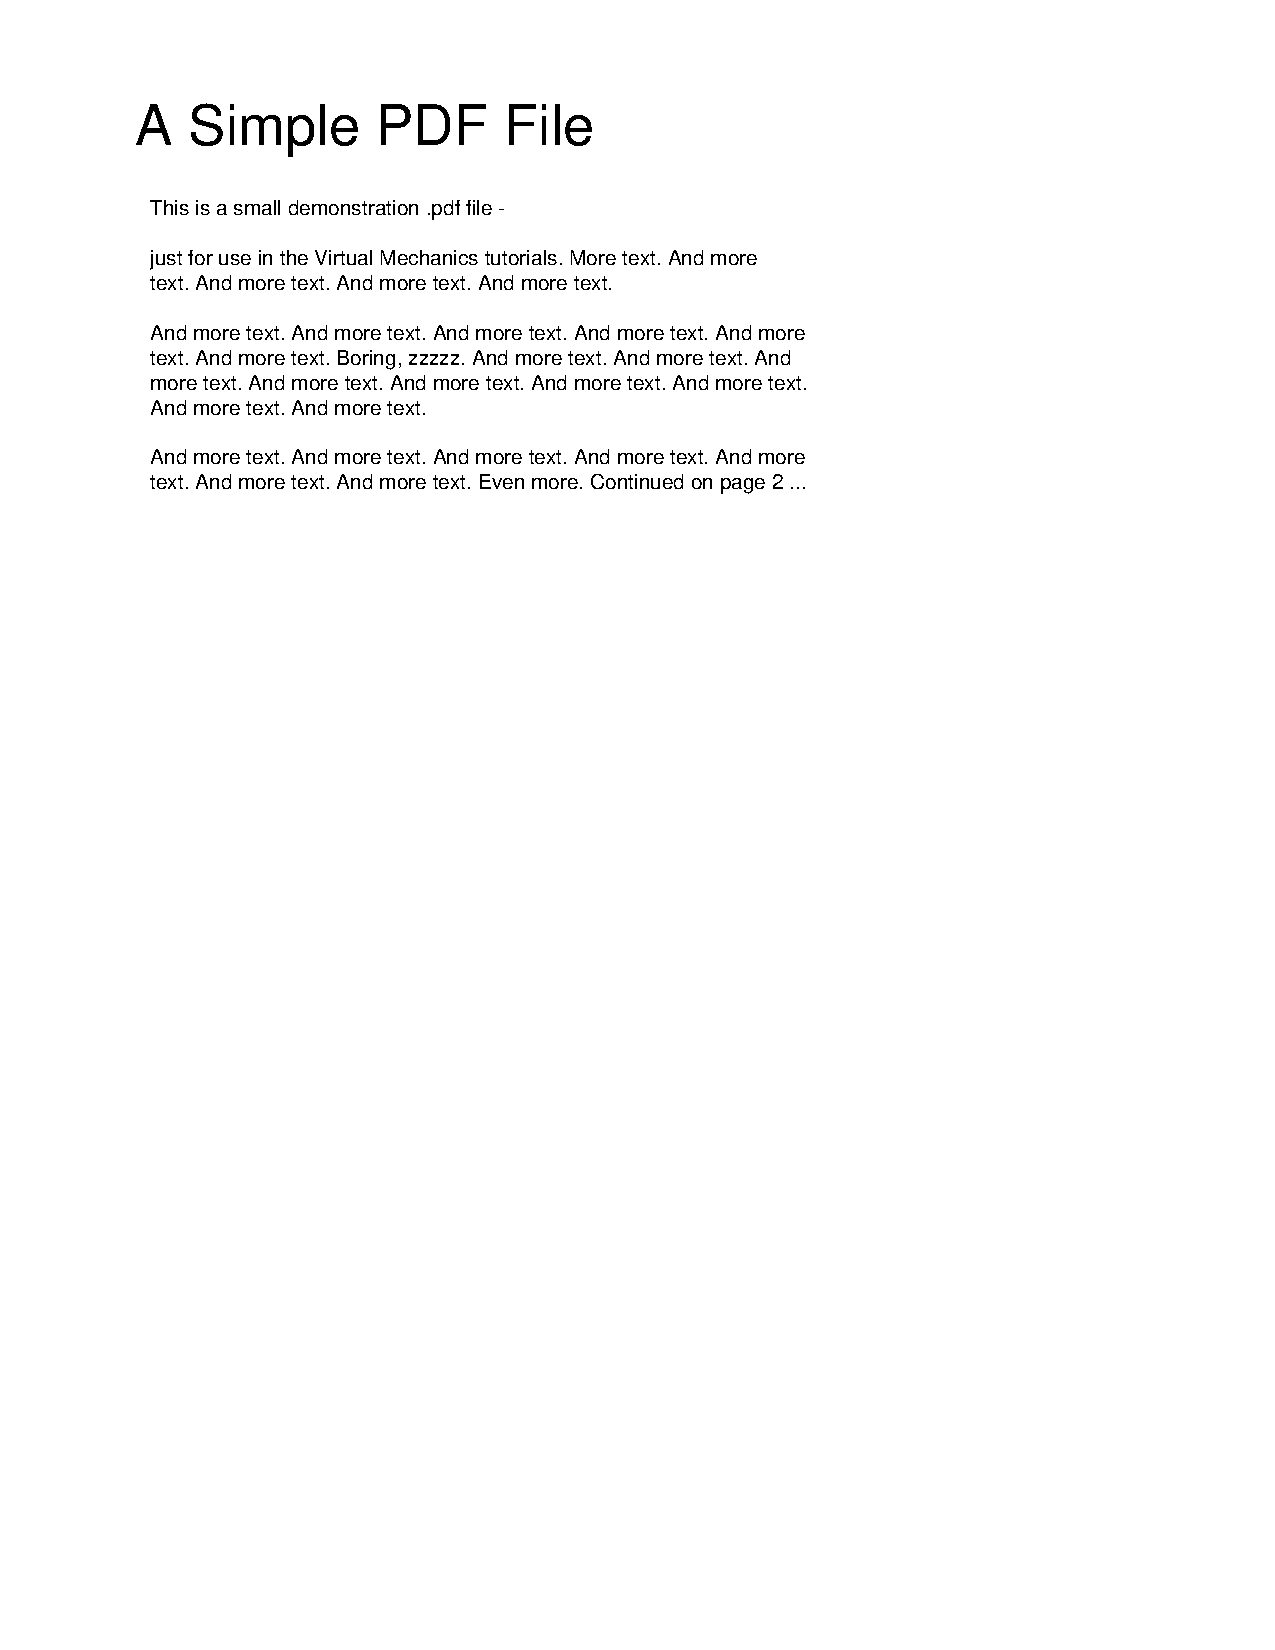
\includepdf[pages=1]{pdf/sample.pdf}
% \end{appendices}



%%%%%%%%%%%%%%%%%%%%%%%%%%%%%%%%%%%%%%%%%imposta l'intestazione di pagina
\renewcommand{\chaptermark}[1]{\markright{\thechapter \ #1}{}}
\lhead[\fancyplain{}{\bfseries\thepage}]{\fancyplain{}{\bfseries\rightmark}}
\appendix                               %imposta le appendici
\chapter{Prima Appendice}               %crea l'appendice
In questa Appendice non si � utilizzato il comando:\\
%%%%%%%%%%%%%%%%%%%%%%%%%%%%%%%%%%%%%%%%%\verb"" � equivalente all'
                                        %   ambiente verbatim,
                                        %   ma si utilizza all'interno
                                        %   di un discorso.
\verb"\clearpage{\pagestyle{empty}\cleardoublepage}", ed infatti
l'ultima pagina 8 ha l'intestazione con il numero di pagina in
alto.
%%%%%%%%%%%%%%%%%%%%%%%%%%%%%%%%%%%%%%%%%imposta l'intestazione di pagina
\rhead[\fancyplain{}{\bfseries \thechapter \:Prima Appendice}]
{\fancyplain{}{\bfseries\thepage}}
\chapter{Seconda Appendice}             %crea l'appendice
%%%%%%%%%%%%%%%%%%%%%%%%%%%%%%%%%%%%%%%%%imposta l'intestazione di pagina
\rhead[\fancyplain{}{\bfseries \thechapter \:Seconda Appendice}]
{\fancyplain{}{\bfseries\thepage}}
\begin{thebibliography}{90}             %crea l'ambiente bibliografia
\rhead[\fancyplain{}{\bfseries \leftmark}]{\fancyplain{}{\bfseries
\thepage}}

% Bibliografia alternativa (usare chapter o section a seconda del tipo di documento)
% \renewcommand{\bibsection}{}
% \chapter*{Riferimenti bibliografici}
% \bibliography{refs} %file .bib

%%%%%%%%%%%%%%%%%%%%%%%%%%%%%%%%%%%%%%%%%aggiunge la voce Bibliografia
                                        %   nell'indice                                     
\addcontentsline{toc}{chapter}{Bibliografia}
%%%%%%%%%%%%%%%%%%%%%%%%%%%%%%%%%%%%%%%%%provare anche questo comando:
%%%%%%%%%%%\addcontentsline{toc}{chapter}{\numberline{}{Bibliografia}}
\bibitem{K1} Primo oggetto bibliografia.
\bibitem{K2} Secondo oggetto bibliografia.
\bibitem{K3} Terzo oggetto bibliografia.
\bibitem{K4} Quarto oggetto bibliografia.
\end{thebibliography}
%%%%%%%%%%%%%%%%%%%%%%%%%%%%%%%%%%%%%%%%%non numera l'ultima pagina sinistra
\clearpage{\pagestyle{empty}\cleardoublepage}
\chapter*{Ringraziamenti}
\thispagestyle{empty}
Qui possiamo ringraziare il mondo intero!!!!!!!!!!\\
Ovviamente solo se uno vuole, non � obbligatorio.
\end{document}
